\chapter{Background}

In this chapter the theoretical foundations and tools for the succeeding work are treated.
Firstly, the MAC layer is introduced in the context of the OSI reference model. Successively, a glance on a number of different MAC protocols and mechanisms is taken, while analyzing weaknesses with respect to the challenges coming up in wireless transmission. The chapter concludes with naming the advantages of software-defined radio.   

\bigskip

\section{MAC Protocols}

\subsection{MAC Layer in the OSI Model}

The OSI model is a layered architecture that divides a telecommunication system into several manageable layers. The original model features seven layers, where the focus in this thesis is on the MAC layer. Nevertheless, each layer's responsibilities is briefly listed. Then, a closer look on different realizations of the MAC layer is taken. Note that the data link layer has been split into two sublayers: the medium access and the logical link control sublayers.

% Sketch of ISO/OSI-model

\begin{table}[h]
	\centering
	\begin{center}
		\begin{tabular}{p{3.5cm}p{10cm}}
			\toprule
				Layer & Responsibilities \\
			\midrule
				Physical Layer & dealing with mechanical, electrical and timing interfaces of data transmission  \\
				MAC Sublayer & controlling medium access and frame synchronization \\
				LLC Sublayer & multiplexing to enable different network protocols coexist, flow control and error control.  \\
				Network Layer & routing and congestion control \\
				Transport Layer & transmission reliability, same-order-delivery, congestion avoidance  \\
				Session Layer & token management, dialog control, synchronization \\
				Presentation Layer & abstracting syntax and semantics of transmission \\
				Application Layer & user application protocols, such as http, ftp, smtp and many more \\
			\bottomrule
		\end{tabular}\caption{Layers in the OSI model} \label{tab:osi-layers}
	\end{center}
\end{table}

\subsection{ALOHA}

ALOHA is arguably the most simple MAC protocol. The basic idea is whenever a user wants to send data he does so. The higher the channel load, i.e. sending requests per time unit, the more likely collisions will occur, which render all transmitted information useless.

\bigskip

The question that comes to mind is, how likely is it that a collision will not occur. In other words, how efficient is an ALOHA channel? Making a statement requires a few preliminary assumptions:

\smallskip

\begin{enumerate}
	\item We are taking a look at pure ALOHA as described above.
	\item We simplify the calculation by assuming a fixed frame length.
	\item The number of packets generated during a frame time is a poisson-distributed random variable $X$.
	\item The channel load $G$ comprises of two portions: "new" and retransmitted frames.
\end{enumerate}

\bigskip

The probability mass function of the Poisson distribution and thus the probability of $k$ frames being generated during a given frame time amounts to:

\begin{equation}
	Pr(X=k) = \frac{G^k\cdot e^{-G}}{k!}
\end{equation}

The probability of zero frames being generated during the transmission of the frame is $Pr(X=0) = e^{-G}$ (assumption 3). If no collision occurs during the transmission of frame $F$ no other frame was sent off during that transmission. Conversely, $F$ itself did not collide with a frame sent off prior to $F$. We conclude that the vulnerability period during which collision may corrupt data is two frame times (assumption 2).

\bigskip

The probability that no frame other than the frame to be transmitted is generated during the two frame time vulnerability period is $P_0 = e^{-2G}$. The throughput $S$ is given by $S=GP_0 = Ge^{-2G}$.

\bigskip

The maximum throughput is achieved when $\frac{\partial S}{\partial G} \stackrel{!}{=} 0$:


\begin{eqnarray}
	& \frac{\partial S}{\partial G} & = \frac{\partial}{\partial G} Ge^{-2G} \\ 
	& & = e^{-2G}(1-2G) \\
	& & \stackrel{!}{=} 0 \\
	\Leftrightarrow & G & = 0.5
\end{eqnarray}
	

\bigskip

This means that for $G=0.5$ the throughput S reaches its maximum $S_\text{ALOHA,max} = \frac{1}{2e} \approx 0.18$. This result is very reasonable, since the transmission of a frame is vulnerable for the duration of two frame times, so the maximum is achieved when sending exactly every second slot, where a slot is equivalent to the frame time.

\bigskip

As an aside, the throughput can be doubled with slotted ALOHA. In contrast to pure ALOHA, slotted ALOHA allows transmission only at the beginning of slots, which effectively halves the vulnerability period to only one slot, since frames transmitted prior to a frame $F$ cannot interfere with $F$ anymore. Thus, $S_\text{ALOHA,max} = \frac{1}{e} \approx 0.36$, reached at $G=1$. However, this comes at the cost of an additional frame delay of $t_\text{slot}$ in the worst case and $\frac{t_\text{slot}}{2}$ in the average case.

\begin{figure}[h]
	\label{fig:aloha-performance}
	\begin{center}
		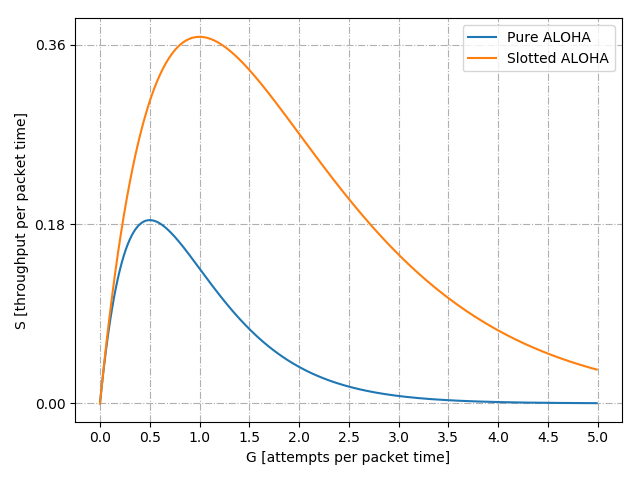
\includegraphics[width=13cm]{pictures/aloha_performance}
	\end{center}
	\caption{Pure ALOHA and slotted ALOHA's performance.}
\end{figure}

As shown above in figure \ref{fig:aloha-performance} and the preceding paragraphs ALOHA's performance is discouraging and improvements over ALOHA were found. 

\subsection{CSMA}

Main problem of ALOHA is the negligence of concurrent traffic in the channel. A solution to this problem is offered by the "listen before talk" (LBT) mechanism, which means in order to avoid collisions we sense the channel and refrain from sending should it be busy. This is the simple, yet effective basic idea of carrier sensing multiple access (CSMA) which comes in three flavors, as depicted in figure \ref{fig:csma-flavors} which will be discussed next.

\begin{figure}[htp] \label{fig:csma-flavors}
	\begin{center}
		\subfloat[1-persitent CSMA]{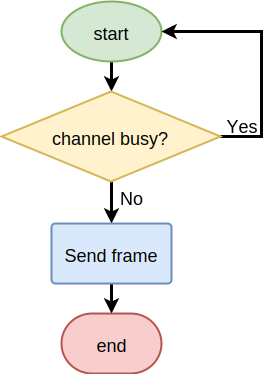
\includegraphics[width=0.22\textwidth]{pictures/csma_1_persistent}}
		\qquad
		\subfloat[non-persistent CSMA]{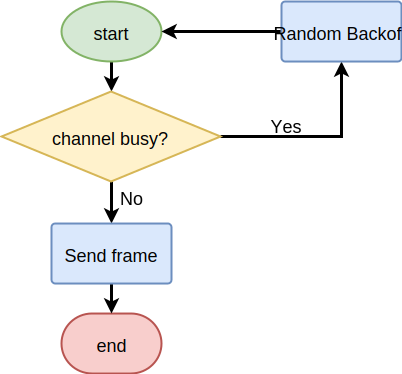
\includegraphics[width=0.31\textwidth]{pictures/csma_non_persistent}}
		\qquad
		\subfloat[p-persistent CSMA]{\includegraphics[width=0.35\textwidth]{pictures/csma_p_persistent}}
	\end{center}
\caption{The three flavors of CSMA}
\end{figure}


\subsubsection{1-persistent CSMA}

% 1-persistent CSMA flowchart

When the channel is busy 1-persistent CSMA waits until the channel becomes idle. As soon as the channel is found idle a frame is transmitted with a probability of 1, hence 1-persistent CSMA. If the frame collides with another, the node waits for a random backoff time and then the whole process is started all over again.

\bigskip

Despite being a substantial improvement over ALOHA, this protocol has at least two problems:

\begin{itemize}
	\item Provided propagation delay is zero or negligible, collisions can still occur.  Imagine a three-node-scenario with nodes $A$, $B$ and $C$. $A$ is transmitting, while $B$ and $C$ are waiting for their turn. Once $A$ finished transmission $B$ and $C$ will lunge onto the channel like a pack of wolves leading to collision.
	
	\item If propagation delay is not negligible the protocol suffers from another problem. In this scenario $A$ has just begun sending. $B$ will assume the channel is idle and send off his frame, since, due to the propagation delay, $B$ has not yet heard of $A$. This is why propagation delay may significantly hamper this protocol's performance.
\end{itemize}  

\subsubsection{Non-persistent CSMA}

% non-persistent CSMA flowchart 

In order to alleviate 1-persistent CSMA's problem with several nodes trying to seize the channel as soon as it becomes idle a less greedy attempt is made with non-persistent CSMA. Instead of continuously sensing the channel until it becomes idle nodes wait a random backoff time until they listen again. As a result, this protocol leads to better channel utilization with the downside of higher delays.

\subsubsection{P-persistent CSMA}

% p-persistent CSMA flowchart

P-persitent CSMA is a protocol for slotted channels. Whenever a node $A$ wishes to send off a packet the channel is sensed. If the channel is found idle it transmits its packet with a probability of $p$. With a probability $1-p$ it defers the transmissions to the next slot. This process is repeated until one either the packet is sent off or the channel is found busy again. In the latter case $A$ acts as though a collision had taken place and waits a random time until starting again.

\bigskip

This flavor of CSMA can be regarded as a compromise between 1-persistent CSMA and non-persistent CSMA, where the choice of $p$ determines the greediness. The smaller $p$, the less greedy and thus the closer p-persistent CSMA approximates non-persistent behavior. An appropriate choice of $p$ can get the best out of both worlds: minimal delays as in 1-persistent CSMA, as well as high channel efficiency as in non-persistent CSMA.

\subsection{CSMA with Collision Detection}

A way to further improve CSMA-family protocols is to immediately cancel transmissions once a collision is detected. There is no point in continuing these transmissions, as the transmitted data is lost in any case. Stating the obvious, aborting transmission saves both bandwidth and time. 

\bigskip

CSMA/CD is used on wired LANs and serves as basis of the wide-spread Ethernet. However, this mechanism is not extensively made use of in wireless networks. Concerning the reason, it is cardinal to understand that collision detection is an analog process. A collision is detected by comparing the received and transmitted signal's energy or pulse width, which premises transmission and reception taking place simultaneously. 

\bigskip

This condition mostly is not met for wireless nodes, which are half-duplex. The reason for this lies in the conservation of energy.

\begin{equation}
	P = \int_{A} I(\vec{x}) \, dA
\end{equation}

Where $P$ is the power, $I$ the intensity as function of the position $\vec{x}$ and $dA$ the differential element of a closed surface around the source. Assuming that the integration takes place over the surface of a sphere with the radius $r$ the term simplifies to:

\begin{eqnarray} 
	& P = & \abs{I(r)} \cdot 4\pi r^2 \\
	\label{eqn:intensity}
	\Leftrightarrow & \abs{I(r)} = & \frac{P}{4\pi r^2} 
\end{eqnarray}

Another, and more common quantity in telecommunications is signal-to-noise ratio (SNR), which is defined as follows, where $P$ is the signal power and $N$ the noise power: 

\begin{equation} \label{eqn:snr}
	SNR [dB] = 10 \, log \left( \frac{P}{N} \right)
\end{equation}

Equations \ref{eqn:intensity} and \ref{eqn:snr} imply if we increase the distance $r$ by $\sqrt{2}$ the signal's intensity halves or lose 3dB in SNR, respectively. To make up for the loss in signal strength we would have to employ expensive signal processing hardware making wireless equipment less affordable. Alternatively, we could increase the transmit power, but this increases interference with other nodes, as well as electricity consumption.  

\subsection{Challenges for Wireless MAC Protocols}

Wireless MAC protocols have to tackle a few problems that do not occur in wired data exchange. Among them are the hidden node and the exposed node problem, which will be discussed by reference to \ref{fig:hidden_exposed_node_problem}. Further challenges, such as energy limitations will also be delineated.

\subsubsection{The Hidden Node and the Exposed Node Problem}

\begin{figure}[ht]
	\label{fig:hidden_exposed_node_problem}
	\begin{center}
		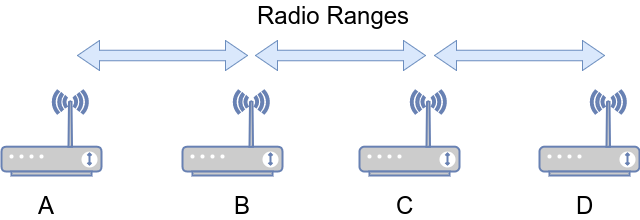
\includegraphics[width=12cm]{pictures/hidden_exposed_node_problem}
	\end{center}
	\caption{Setup to explain the hidden and exposed node problem. Each node can only reach its neighbors.}
\end{figure}

Suppose that the node's radio range is limited to the neighboring nodes and $A$ would like to transmit to $B$. If $C$ just started transmitting $A$ won't hear $C$ and falsely assume that the channel is idle and start transmitting. This is the hidden node problem.

\bigskip

For the same configuration, in another scenario $B$ would like to send to $A$ and $C$ is already transmitting to $D$. $B$ refrains from sending despite collisions would only take place between $B$ and $C$, where it does not matter. This is the exposed node problem. 

\bigskip

\subsubsection{Further Challenges}

% Citation needed for verification
Further challenges to MAC protocol design include the power conservation when faced with constrained power resources, as in wireless sensor networks (WSN) where devices rely on batteries for their supply with power. Attempts to mitigate waste of energy have been made in several specialized, duty-cycle based MACs such as Sensor MAC, Timeout MAC and Berkley MAC.

\bigskip

On the same page, due to constrained energy resources, WSN are especially susceptible to denial of sleep attacks, a special form of denial of service (DoS) attack, drastically increasing energy consumption and thus reducing the system's lifetime. It is due to this fact that security is paramount in biomedical or military fields of application. 

\subsection{CSMA with Collision Avoidance}

802.11 is a set of physical layer (PHY) and MAC specifications for wireless local area networks (WLANs). When the dominant mode of operation, the so-called distributed coordination function (DCF) is employed CSMA/CA is used in the MAC layer.

\bigskip

Beside physical carrier sensing previously simply referred to as carrier sensing another mechanism, namely virtual carrier sensing in combination with RTS/CTS exchange is employed to mitigate the trouble caused by hidden nodes. 

\bigskip

In order to explain these mechanisms we refer to the setup of figure \ref{fig:hidden_exposed_node_problem} with a slight modification in so far as that each node's radio range shall span across two neighboring nodes in both directions. That is to say, $A$ can hear $B$ and $C$, but not $D$ and so on. Figure \ref{fig:virtual_carrier_sensing} visualizes the chain of events whose explanation follows.

\bigskip

\begin{figure}[ht]
	\label{fig:virtual_carrier_sensing}
	\begin{center}
		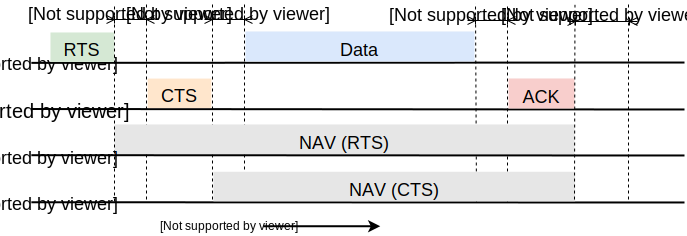
\includegraphics[width=14cm]{pictures/virtual_carrier_sensing}
	\end{center}
	\caption{Virtual Carrier Sensing in CSMA/CA}
\end{figure}

$A$ wants to send to $B$, hence issues a request to send (RTS). Every node receiving the RTS is shut down, except for $B$ that in response to the RTS creates a clear to send (CTS) frame. Not only $A$ receives this CTS frame, but also $D$, a hidden node from $A$'s point of view. Upon reception of CTS $D$ is silenced as well. Therefore, RTS/CTS is addressing the hidden node problem. RTS/CTS are frames of 30 bytes length containing the length of the frame in this case $A$ wants to transmit. Based on this length $C$ and $D$ setup the so-called network allocation vector (NAV), which are node-internal timers reminding $C$ and $D$ that the channel is still in use. Due to the fact, that no physical process is running to detect the channel status this mechanism get its name virtual carrier sensing. Shutting down nodes has the beneficial side-effect of reducing overhearing and therefore reduces energy consumption.

\bigskip

As further depicted in figure \ref{fig:virtual_carrier_sensing} there are named intervals of specified length between each of the frames. Varying lengths of these interval types serve the purpose of prioritizing certain frames over others. 

\medskip
The short interframe spacing (SIFS) is the interval until the next control frame or next fragment (of a fragmented data frame) may be sent. SIFS is designed to allow one party out of the two parties in dialog send off their frame without interference by another node. 

\medskip
The longer interval DCF interframe spacing (DIFS) is the interval after which any station may try to seize the channel for their transmission.

\medskip
For the sake of completeness, we briefly mention two consciously left out intervals, namely point coordination function interframe spacing (PIFS) and extended interframe spacing (EIFS). If 802.11 is operated in an alternative mode of operation, where a base station acts as a coordinator of traffic the standard prescribes an interval of length PIFS to allow the base station to send certain control (beacon and poll) frames. EIFS is used to report the reception of a bad or unknown frame and due to this action's low priority is the longest interval among the mentioned four. 

\bigskip

As a remark on the exposed node problem: MAC protocols such as MACA that feature the RTS/CTS exchange, but no ACK from the receiver also solve the exposed station problem. The inclusion of the ACK however "resurrects" the exposed station problem, since the receiver's ACK can now interfere with node's that are out of the sender's range. However, renouncing on ACKs was dropped in the revised version MACAW, because the absence of lost frames was not noticed until much later in the transport layer, causing huge drops in throughput.

\subsection{Duty-Cycle-Based MAC Protocols}  

... Sensor MAC, Timeout MAC, Berkley MAC ...

\section{Software Defined Radio}
 
\subsection{Purpose of Software Defined Radio}

% figure of fm/am radio electrical circuits
Traditional radio equipment is "hardware-defined", i.e. that the signal processing runs on a specialized electrical circuit.

\subsection{GNU Radio}


